\documentclass[journal]{IEEEtran}

\usepackage[T1]{fontenc}
\usepackage{amsmath,amssymb}
\usepackage{graphicx}
\usepackage{booktabs}
\usepackage{multirow}
\usepackage{siunitx}
\usepackage{tikz}
\usepackage{pgfplots}
\pgfplotsset{compat=1.17}
\usetikzlibrary{shapes.geometric,arrows.meta,positioning,fit}
\usepackage{algorithm}
\usepackage{algpseudocode}
\usepackage{url}
\usepackage{xcolor}

\sisetup{detect-weight=true, detect-family=true}

\begin{document}

\title{From Feasibility to a Measured Timetable: A Taasika-to-UniTime Pipeline at a Computer Engineering Department}

\author{Mihir~Shah, Riya~Kulkarni, Ved~Mundhada, and Akshay~Sathaye\\
\textit{Department of Computer Engineering, COEP Technological University, Pune, India}\\
\textit{Guide: Abhijit A.\ M.}}

\markboth{Preprint, COEP Technological University}{Shah \MakeLowercase{\textit{et al.}}: Taasika-to-UniTime Pipeline}

\maketitle

\begin{abstract}
University course timetabling is an NP-hard assignment problem in which classes, instructors, student cohorts, and rooms must be placed in a weekly grid under hard and soft constraints. An earlier feasibility study showed that UniTime, an open-source scheduler built on the CPSolver library, could express every scheduling rule of a Computer Engineering department without relaxation, but it did not produce a timetable from institutional data. This paper reports the phase that closed that gap. A reproducible pipeline converted a snapshot of the department’s scheduling database into the sixteen ordered XML documents required by UniTime’s Data Exchange interface, covering one academic session, 56 course offerings comprising 291 classes, 115 instructors, 42 rooms, and 1,130 simulated students with 9,148 section enrolments. An independent evaluator, cross-validated against a second Java-based implementation to exact agreement, recomputes conflict counts from the exported timetable and the enrolment file. Several reported zeros were artifacts of silent re-sectioning, an already-solved instance, or an empty student population. With enrolments pinned in the Spr10--Spr12 solves, the final solution placed 290 of 291 classes with no instructor or room double-booking and achieved a hard feasibility score of 98.85 out of 100. Forty of the 1,130 students had a genuine timetable clash, all first-year students in one laboratory-lecture pairing. A reinforcement-learning layer that selected among eight CPSolver neighbourhood operators was also implemented. The 25\% bar was committed on 28 September 2026 (\texttt{6bf9970}) for a learned policy against a tuned baseline on a held-out instance. The weight sweep is not that comparison, and the learned-policy run was never made, so no claim is made that learning outperforms a tuned baseline.
\end{abstract}

\begin{IEEEkeywords}
course timetabling, constraint programming, UniTime, CPSolver, iterative forward search, student conflicts, reinforcement learning.
\end{IEEEkeywords}

\section{Introduction and Problem Statement}
\label{sec:intro}

A university timetable is, at bottom, a very large pile of classes that must each land somewhere in a weekly grid. Every class brings its own room, its own instructor and its own duration, and a long list of hard and soft constraints decides which landings count as acceptable. The problem is NP-hard. No polynomial-time exact algorithm is known, so working systems lean on heuristic or metaheuristic search~\cite{schaerf1999survey}.

The Department of Computer Engineering at COEP Technological University is a stubborn instance. It runs four undergraduate years and a postgraduate programme, each cut into lecture divisions and then into laboratory batches. On top of that sit departmental electives, minor-degree courses taught by other departments, open electives, and reserved first-year blocks. Laboratory sections of a course run in parallel, while its lectures run jointly. The natural scheduling unit is therefore neither the course nor the student but the section, and it is the relationships between sections that make a timetable usable or useless.

An earlier feasibility study evaluates UniTime, an open-source, web-based scheduling system built on the CPSolver constraint library. It deploys the system locally, enters representative test data, and maps the institution's rules onto UniTime's constraint model. Its conclusion is that every identified rule is expressible, with no relaxation and no external post-processing. But that is a claim about a platform, not about a timetable. No institutional data is loaded at that stage, no solution comes from real course structure, and nothing measures solution quality. The data pipeline, the student records and the evaluation framework all remain promises.

Closing that gap matters beyond one department. A model that can \emph{express} every rule says nothing about three further questions. Can a real snapshot of a real scheduling database become solver input without manual re-entry? Is the resulting schedule good by any measure the institution cares about? Can that measure be trusted at all? Each has a less obvious answer than expected, and the third takes up most of this paper. A scheduler that quietly reports a better number than the timetable deserves is arguably worse than one that honestly reports a mediocre one, because the first invites a decision-maker to stop looking for a problem that is still there.

The present phase, run under the project name \emph{taasika-v3}, closes the gap. It contributes the following.
\begin{enumerate}
\item A reproducible pipeline reads a snapshot of the department's existing \emph{Taasika} scheduling database and emits the sixteen ordered XML documents that UniTime's Data Exchange interface consumes.
\item Institution-specific rules are encoded as generated preference data rather than entered by hand. These are the minor-degree and open-elective time blocks and the division and batch structure. The lunch window is not re-entered with that data: a Jython script run inside UniTime writes its solver-parameter definitions into the UniTime database before the timetable solver is run.
\item An independent evaluation framework scores any exported timetable against the same input data. A solver's own quality report cannot audit the solver, so the check has to live outside it.
\item An honest account of solution quality. Several configurations report zero student conflicts, and each turns out to be an artefact rather than an improvement. A final, pinned-enrolment solution is reported in their place.
\item A reinforcement-learning layer that chooses among stock CPSolver neighbourhood operators. The 25\% bar for that layer was committed on 28 September 2026 (\texttt{6bf9970}) and applies to a learned policy on a held-out instance. That comparison was not run.
\end{enumerate}

\subsection{Related work}
Automated timetabling has a long history as a constraint-satisfaction and optimisation problem. Surveys of the field keep returning to constraint programming and local search as the dominant methodologies for university course timetabling, largely because both can mix mandatory and preferential requirements in a single model~\cite{schaerf1999survey}. UniTime and its embedded solver, CPSolver~\cite{cpsolver}, are one mature example. CPSolver combines Iterative Forward Search with Conflict-based Statistics~\cite{muller2004constraint} and does well in international timetabling competitions~\cite{muller2009itc,muller2025itc}. The minimal-perturbation formulation that grows up beside it addresses a very practical need: a re-solved timetable should disturb as few existing placements as possible~\cite{muller2007minimal}. Murray, M\"uller and Rudov\'a set out how an institution's offerings, subparts and sections map onto the model~\cite{murray2007modeling}. Later accounts describe the same system in daily use~\cite{rudova2011complex}, including elective courses and multiple sections~\cite{muller2016curriculum}. Soft requirements enter as weighted criteria, not as extra hard constraints~\cite{rudova2003soft}.

The published literature says much less about two things. One is the \emph{operational} route from an institution's own legacy database into such a system. The other, and the more worrying, is how easily a scheduler's reported conflict count can be made to look better than the timetable really is once students may move between sections. This second gap, not any weakness in the constraint model, is what the paper is about. The feasibility phase already shows the model is adequate. What remains open is whether a working pipeline can be built on it, and whether its output can be measured honestly.

\subsection{Scheduling model}
In the CPSolver model the decision variable is a class, meaning a single lecture, laboratory or tutorial section. Its value is a placement: a start time plus the room or rooms where the class meets. Students are not variables. A student's timetable falls out of the placements chosen for the classes that student attends, and an overlap between two classes is priced through a joint-enrolment constraint between them. So the solver has only two ways to improve a student's timetable. It can move a class, or, if allowed, it can move the student into a different section. The second route is the one that later sections expose as a source of illusory improvement. Student sectioning is a problem in its own right~\cite{muller2010sectioning}, not a side effect of timetabling.

Hard constraints hold in every acceptable timetable. No room or instructor hosts two overlapping classes. A class sits only in a room whose capacity and type suit it. Every class respects its declared meeting pattern and the term's date pattern, and weekends are excluded. Soft constraints describe quality rather than legality: preferred rooms and times, balanced instructor load, limited back-to-back teaching, a protected lunch window, and, the one this paper treats as primary, the number of students whose personal timetable contains an overlap.

\subsection{The measurement problem}
\label{sec:measurement-problem}
Producing a feasible timetable is not the hard part here. Coverage, room and instructor feasibility arrive early. The hard part is that student-conflict counts cannot be trusted, because three separate mechanisms push the reported figure toward zero without helping any student.

The first is \emph{re-sectioning}. UniTime shuffles students between parallel laboratory batches until the overlaps vanish, while the placements themselves never change. The second is an \emph{empty student population}: a demand setting that loads zero students reports zero conflicts over an empty denominator. The third is a \emph{denominator mismatch}. A conflict rate computed over the students who carry enrolments in a solver export is simply not comparable to one computed over every student in the source data.

Sections~\ref{sec:evaluator} and~\ref{sec:results} therefore treat the task as two objectives, not one. First, produce a feasible timetable. Second, establish a measurement of student conflicts that none of these three mechanisms can satisfy.

\subsection{Solver mechanics}
CPSolver is a local-search framework with constraint-programming primitives, built on Iterative Forward Search (IFS)~\cite{muller2004constraint}. IFS departs from classical local search in one respect: it works over solutions that are feasible but possibly incomplete. Some classes may stay unassigned, yet every hard constraint holds for those that are assigned, so an intermediate solution always makes sense to a human scheduler. Starting from an initial timetable, each iteration picks a class and a placement, removes the assignments that hard-conflict with it, installs the new one, and remembers the best timetable seen so far.

Fig.~\ref{fig:ifs} shows the loop as it runs in this project, including the difference between proposing a move and committing it. The reinforcement-learning layer of Section~\ref{sec:rl} replaces only the \emph{Propose move} step. That step draws one assignment from the neighbourhood of the current one, the mechanism M\"uller describes in his thesis~\cite{muller2005thesis}. CPSolver exposes the neighbourhood choice through its \texttt{NeighbourSelection} extension point. The competition solver's time changes, room changes and swaps appear in~\cite{muller2009itc}, and later changes to that set in~\cite{muller2016evolution}. A great-deluge rule decides whether a proposed move is accepted~\cite{dueck1993deluge}.

IFS is further augmented with Conflict-based Statistics (CBS)~\cite{muller2004constraint}. CBS records how often each assignment has historically caused a hard conflict with another, and during value selection it penalises candidate placements accordingly. The search drifts away from historically troublesome regions. Throughout, \texttt{Basic.DisobeyHard} is \texttt{false}, so every mechanism described later inherits the guarantee that a persisting assignment never violates a hard constraint.

\begin{figure}[t]
\centering
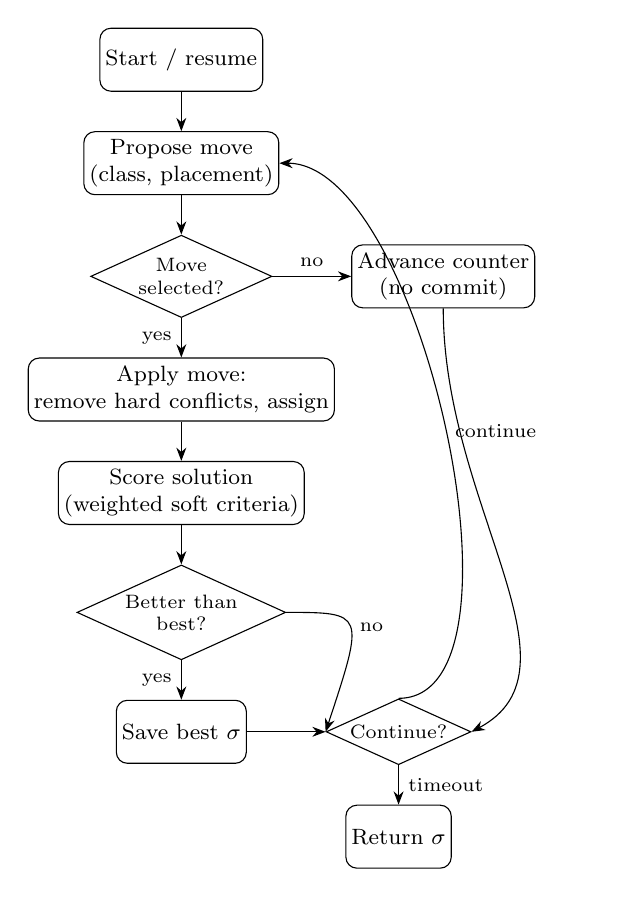
\begin{tikzpicture}[
    node distance=5mm and 6mm,
    box/.style={draw, rounded corners, align=center, minimum height=8mm, font=\footnotesize, inner sep=2pt},
    dec/.style={draw, diamond, aspect=2.2, align=center, font=\scriptsize, inner sep=1pt},
    >=Stealth
]
\node[box] (start) {Start / resume};
\node[box, below=of start] (propose) {Propose move\\(class, placement)};
\node[dec, below=of propose] (hasmove) {Move\\selected?};
\node[box, below=of hasmove] (apply) {Apply move:\\remove hard conflicts, assign};
\node[box, below=of apply] (score) {Score solution\\(weighted soft criteria)};
\node[dec, below=of score] (better) {Better than\\best?};
\node[box, below=of better] (save) {Save best $\sigma$};
\node[box, right=10mm of hasmove] (advance) {Advance counter\\(no commit)};
\node[dec, right=10mm of save] (cont) {Continue?};
\node[box, below=of cont] (ret) {Return $\sigma$};

\draw[->] (start) -- (propose);
\draw[->] (propose) -- (hasmove);
\draw[->] (hasmove) -- node[left, font=\scriptsize]{yes} (apply);
\draw[->] (hasmove) -- node[above, font=\scriptsize]{no} (advance);
\draw[->] (apply) -- (score);
\draw[->] (score) -- (better);
\draw[->] (better) -- node[left, font=\scriptsize]{yes} (save);
\draw[->] (save) -- (cont);
\draw[->] (better.east) .. controls +(10mm,0) .. node[right, font=\scriptsize]{no} (cont.west);
\draw[->] (advance.south) .. controls +(0,-25mm) and +(15mm,8mm) .. (cont.east);
\draw[->] (cont) -- node[right, font=\scriptsize]{timeout} (ret);
\draw[->] (cont.north) .. controls +(18mm,0) and +(18mm,0) .. node[right, font=\scriptsize]{continue} (propose.east);
\end{tikzpicture}
\caption{The CPSolver Iterative Forward Search loop as configured in this project. The incumbent $\sigma$ is updated only when the comparator judges the new solution better. The reinforcement-learning layer of Section~\ref{sec:rl} substitutes only the \emph{Propose move} step.}
\label{fig:ifs}
\end{figure}

UniTime models a course hierarchically. An instructional offering carries one or more configurations, each configuration holds scheduling subparts (a lecture subpart and a laboratory subpart, say), and each subpart holds the classes that actually get placed. This hierarchy lets a course with joint lectures and parallel laboratory batches live as a single offering. It also explains why the institution's division-and-batch structure maps onto UniTime without distortion.

\section{Data and Institution-Specific Constraints}
\label{sec:data}

\subsection{Source system and pipeline}
\emph{Taasika} is the scheduling database the institution already uses. A SQL dump of it holds the data as a run of numbered snapshots, each a complete picture of the departmental schedule at one moment. The pipeline parses that dump as text instead of restoring it into a database server. This is deliberate. The loader reads the dump and exposes each table as a list of records filtered to a chosen snapshot, so nothing downstream depends on a database, and the dump stays immutable input.

Fig.~\ref{fig:pipeline} traces the whole path from SQL dump to scored timetable. Eight generator modules run in dependency order and cover the session, curriculum structure, rooms, instructors, course offerings, scheduling preferences and a simulated student body. Three validators check the result, and an archive step produces the ZIP file that UniTime's Data Exchange page accepts. The sixteen documents must go in a fixed order, since each later file points at entities an earlier one creates. The time-pattern and date-pattern preferences matter most here. They have to precede the student records, or UniTime treats the classes as ``arrange hours'' and never loads them into the solver at all.

\begin{figure}[t]
\centering
\resizebox{\linewidth}{!}{%
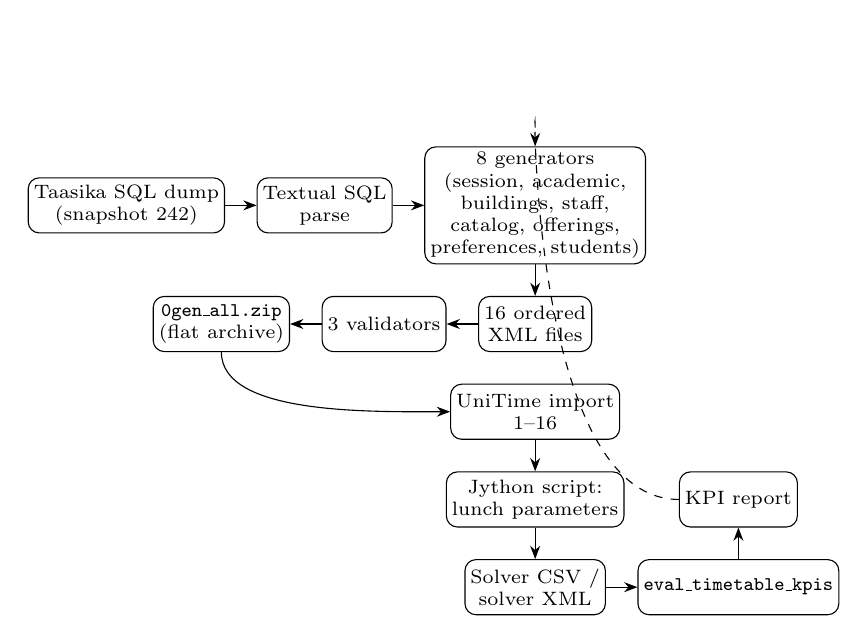
\begin{tikzpicture}[
    node distance=4mm and 4mm,
    box/.style={draw, rounded corners, align=center, font=\scriptsize, inner sep=2pt, minimum height=7mm},
    >=Stealth
]
\node[box] (sql) {Taasika SQL dump\\(snapshot 242)};
\node[box, right=of sql] (loader) {Textual SQL\\parse};
\node[box, right=of loader] (gen) {8 generators\\(session, academic,\\buildings, staff,\\catalog, offerings,\\preferences, students)};
\node[box, below=of gen] (xml) {16 ordered\\XML files};
\node[box, left=of xml] (val) {3 validators};
\node[box, left=of val] (zip) {\texttt{0gen\_all.zip}\\(flat archive)};
\node[box, below=of xml] (import) {UniTime import\\1--16};
\node[box, below=of import] (lunch) {Jython script:\\lunch parameters};
\node[box, below=of lunch] (export) {Solver CSV /\\solver XML};
\node[box, right=of export] (eval) {\texttt{eval\_timetable\_kpis}};
\node[box, above=of eval] (report) {KPI report};

\draw[->] (sql) -- (loader);
\draw[->] (loader) -- (gen);
\draw[->] (gen) -- (xml);
\draw[->] (xml) -- (val);
\draw[->] (val) -- (zip);
\draw[->] (zip.south) .. controls +(0,-8mm) and +(-10mm,0) .. (import.west);
\draw[->] (import) -- (lunch);
\draw[->] (lunch) -- (export);
\draw[->] (export) -- (eval);
\draw[->] (eval) -- (report);
\draw[->, dashed] (report.west) .. controls +(-20mm,0) and +(0,15mm) .. (gen.north);
\end{tikzpicture}}
\caption{The taasika-v3 pipeline. Data flows from the SQL snapshot to a scored timetable. The Jython step writes the lunch parameters before the solve. The dashed return path is the refinement loop of Section~\ref{sec:evaluator}.}
\label{fig:pipeline}
\end{figure}

\subsection{Dataset}
The working dataset, \texttt{unitime-out/0gen\_all}, carries the term attribute \texttt{Spr12} and year 2026 throughout, which gives the Data Exchange term identifier \texttt{Spr122026}. It comes from Taasika snapshot 242, named \texttt{published-v4-26jan26}. The label alone is not enough to settle this, so the snapshot is identified by cross-checking entity counts against the source database. Four documents still carry a hard-coded \texttt{created} attribute naming snapshot 240: session setup, room sharing, travel times, and course offerings. That string is stale. Snapshot 242 is the one the entity counts match, and every figure in this paper uses it.

Table~\ref{tab:inventory} gives the inventory, recomputed directly from the generated files.

\begin{table}[t]
\centering
\caption{Inventory of \texttt{unitime-out/0gen\_all} (term Spr122026).}
\label{tab:inventory}
\footnotesize
\begin{tabular}{@{}ll@{}}
\toprule
File & Contents \\
\midrule
1sessionSetup & session, departments, subject areas, patterns \\
2academicArea & 2 areas (B.Tech, M.Tech) \\
3academicClassification & 5 year codes (FY, SY, TY, BT, MT) \\
4Major / 5Minor & 15 majors; minors modelled as majors \\
6studentGroup & 242 groups (43 classes + 199 batches) \\
7buildingRoomImport & 6 buildings, 42 rooms \\
8roomSharing & 45 sharing blocks; weekends unavailable \\
9travelTimes & 7 inter-building travel entries \\
10staff & 115 instructors \\
11courseCatalog & 158 courses \\
12courseOffering & 56 offerings, 84 subparts, 291 classes \\
13preferences & 362 preference blocks \\
14studentInfo & 1{,}130 students, 5{,}767 group refs. \\
15studentRequest & requests for 1{,}130 students \\
16studentenrollments & 9{,}148 section enrolments \\
\bottomrule
\end{tabular}
\end{table}

Table~\ref{tab:population} describes the simulated student population. Institutional MIS data is not available, so the student body is built from headcounts confirmed with the department. The simulation allocates students to lecture divisions, then to laboratory batches. It then issues a course request for every compulsory subject and one per elective group, and finally enrols each student in a concrete lecture and laboratory section. No real student data appears anywhere in the dataset. Every identifier is synthetic.

\begin{table}[t]
\centering
\caption{Simulated student population of the current dataset.}
\label{tab:population}
\footnotesize
\begin{tabular}{@{}lrrl@{}}
\toprule
Year & CSE & AI\&ML & Total / structure \\
\midrule
First year (FY) & 300 & 100 & 400, single cohort \\
Second year (SY) & 200 & 0 & 200, two lecture divisions \\
Third year (TY) & 200 & 0 & 200, two divisions \\
Final year (BT) & 200 & 0 & 200, two divisions \\
M.Tech (MT) & \multicolumn{2}{c}{130} & specialization streams \\
\midrule
Total & \multicolumn{2}{c}{} & \textbf{1{,}130}, all with enrollments \\
\bottomrule
\end{tabular}
\end{table}

\subsection{Institution-specific constraints as generated data}
The mapping from institutional rule to UniTime construct comes out of the earlier feasibility phase. It shows that a rule \emph{can} be expressed, and that is all it shows, since it schedules nothing. The job in this phase is to generate the matching preference data for every class in the dataset. The time-block rules then reproduce themselves on each pipeline run, with no re-entry by hand after an import.

The institution reserves fixed windows in the week for course categories taught across departments. Minor-degree courses meet on Monday and Tuesday evenings, and open electives on Monday and Tuesday mornings. These are hard commitments, and they have a second half that is easy to miss. Reserving a window for one category achieves nothing unless every other course is kept out of it. A small rule engine handles both halves. It is consulted for every scheduling subpart, and the first rule whose course pattern matches, and whose exclusion pattern does not, becomes active for that subpart. Table~\ref{tab:blocks} lists the four rules in force.

\begin{table}[t]
\centering
\caption{The fixed time-block rules, in evaluation order.}
\label{tab:blocks}
\footnotesize
\begin{tabular}{@{}lllc@{}}
\toprule
Rule & Days & Window & Level \\
\midrule
MDM required & Mon, Tue & 16:30--18:30 & Required \\
OE required & Mon, Tue & 09:30--10:30 & Required \\
Non-MDM prohibited & Mon, Tue & 16:30--18:30 & Prohibited \\
SY non-OE prohibited & Mon, Tue & 09:30--10:30 & Prohibited \\
\bottomrule
\end{tabular}
\end{table}

A required rule pins one slot matching the day set and window to a matching course. A prohibited rule clears every other candidate class whose days and interval overlap the window. Rules run in the order shown, and only the first applicable one governs a given subpart, so a course that happens to match two patterns still answers to a single rule. The second-year prohibition is written course by course, not by wildcard, because only that year's core subjects share the open-elective morning.

The dataset also declares 242 student groups, one for each class and each laboratory batch, and every student joins the groups matching the classes they attend. This makes the cohort structure visible in the UniTime interface and is a prerequisite for a possible future group reservation. It does not, by itself, constrain the timetable. With student switching disabled, as Section~\ref{sec:final} requires, a student's groups only affect a distance computation for students not yet enrolled, and the final sectioning pass never reads them. What really pins a student to a section is the enrolment file together with the three solver settings of Section~\ref{sec:final}. The group data is informative, not load-bearing, and adding it changes no placement and no conflict count. Laboratories jointly supervised by two instructors for one batch use UniTime's native support for multiple lead instructors on a single class, the same mechanism the pipeline already uses to emit one laboratory class per batch record.

The dynamic one-hour lunch break falls between 11:30 and 15:30 and applies separately to students and to instructors. It is not generated preference data. A Jython script run inside UniTime writes the solver-parameter definitions into the UniTime database, and it is run before the timetable solver, rather than as a blocked slot in the time patterns. A universal blocked hour would remove the same window from every day for every class, whereas the institution wants only that each person has \emph{some} free hour inside the window. The criterion is soft, so the solver may violate it. Section~\ref{sec:results} reports how often it does.

\subsection{Translating a legacy schema}
Translating Taasika into UniTime also means resolving a handful of structural mismatches between the two data models. None is a scheduling rule in the sense of Table~\ref{tab:blocks}, yet each decides whether the generated data is interpretable by the solver at all.

A laboratory or tutorial subject is merged into its lecture partner whenever its short name is the lecture's short name plus a recognised suffix. A joint lecture and its parallel laboratory batches then become one offering with two scheduling subparts, not two unrelated courses. Credits follow the local engineering convention: one credit per weekly lecture hour, half a credit per laboratory hour. Unpaired subjects fall back to the lecture-only or laboratory-only half of the same formula, with a floor of one credit. Class identifiers are built to be readable and stable, made of an area code, a course number, a type and a suffix. The student-enrolment documents reference exactly these identifiers, so an unstable scheme would quietly break the dependency chain in Table~\ref{tab:inventory}.

Taasika records room names but not buildings. A heuristic on room and subject short names therefore assigns each room to one of six inferred buildings. Laboratories that are not actually usable go into a separate pool, so any use of them stays visible in the evaluation and cannot hide among normal rooms. Instructor rank is derived from each teacher's declared minimum- and maximum-hours envelope, because Taasika has no rank field.

Last, and most important for Section~\ref{sec:evaluator}, no class carries an explicit time in the generated data. The existing Taasika timetable rows are deliberately not imported as time preferences. The aim is for UniTime to solve the timetable from scratch, not to reproduce the hand-built one. Room associations from Taasika are likewise emitted as preferences, not pre-assignments, so the solver is free to place each class in any suitable room.

\subsection{Identifying the source snapshot}
The Taasika dump stores many numbered snapshots, and the generated XML's own provenance string proves unreliable. Which snapshot produced the working dataset therefore has to be settled by evidence, not by a label. Table~\ref{tab:snapshot} compares three candidates against the final dataset on three counts the generators carry over almost unchanged from the source: student groups (one per class plus one per laboratory batch), teachers, and rooms. Snapshot 242 matches the working dataset exactly on groups and staff. An earlier snapshot (240) and a later one (263, integrated into the loader for the following academic year but not used here) do not.

The room count needs a word of explanation. The raw snapshot holds 49 rooms, but the pipeline no longer emits a virtual ``online'' building. Taking away seven online rooms leaves the 42 that are actually imported, which is why Table~\ref{tab:inventory} shows 42.

\begin{table}[t]
\centering
\caption{Identifying the source snapshot by counting entities.}
\label{tab:snapshot}
\scriptsize
\begin{tabular}{@{}lrrrr@{}}
\toprule
Quantity & Snap 240 & Snap 242 & Snap 263 & 0gen\_all \\
\midrule
Classes+batches=groups & 208 & 242 & 160 & 242 \\
Teachers & 113 & 115 & 67 & 115 \\
Rooms (raw/imported) & 49 & 49 & 29 & 42 \\
\bottomrule
\end{tabular}
\end{table}

\subsection{Student simulation and its consequences}
A course timetable can be produced without students, since the solver needs only classes, rooms, instructors and preferences. Evaluating one is another matter. The criterion the institution cares about most has no meaning until every student is attached to a concrete set of sections. The simulation is not random. It starts from the confirmed headcounts of Table~\ref{tab:population} and allocates students to lecture divisions, then to laboratory batches within a division. It issues a course request for every compulsory subject of that year and one per elective group, then enrols each student in a concrete lecture section and a concrete laboratory section. That last step yields the 9{,}148 enrolment rows of Table~\ref{tab:inventory}.

Enrolment goes section by section. A student is placed in the preferred section for their division until it reaches its declared limit, and after that the routine spills into later sections of the same course and type, much as an over-subscribed laboratory is handled in practice. Two visible consequences follow in the generated data, and both belong to the input, not the solver. First, a few laboratory batches end up mixed, with students from two different lecture divisions, because one division's preferred batches filled first. Three final-year batches are like this. Second, where the declared limits do not cover a cohort at all, the generator reports the unplaced students instead of silently dropping them. That is the origin of the two over-subscribed postgraduate laboratory places revisited in Section~\ref{sec:discussion}.

A genuine timetable overlap has to be distinguished from an artefact of one of these cross-division batches before either consequence can be read on its own.
\section{Evaluation Framework and the Conflict Rule}

\label{sec:evaluator}

There are solution summaries from solver states in UniTime, and we couldn't rely solely on those internal fields, as it results in blind spots. An example of this was with zero conflicts; if it switches students into different sections during the solve, it again reports zero conflicts. Inconsistency between the solver's conflicts and our script to measure conflicts was evident.

To check schedules independently, we created a standalone Python evaluator (eval\_timetable\_kpis) that takes an exported timetable and the source XML directory as inputs and computes the metrics from scratch. In CSV mode, student membership comes from the input enrolment file and meeting times come from the exported solution.

The evaluator operates in two modes,
\begin{itemize}
  \item CSV mode evaluates a timetable exported from the UniTime Web Interface and joins the exported class times to the enrolment XML, and
  \item XML mode evaluates a CPSolver backup XML, that bundles rooms, classes, constraints, placements and the solver’s internal student records.
\end{itemize}

Two classes conflict for a student only when they share a day, their time intervals overlap (a shared endpoint does not count), and, if both have a date pattern, they share an active week. We don't even look at which room is allotted or which teacher is taking the class when checking for a clash. To make sure our logic was actually working properly, we coded the exact same thing in two different language: once in Python for the offline checker, and again in Java for the conflict oracle in the RL part (Section \ref{sec:rl}). When we ran both of them on the same sample solution, the Java one gave a rate of $0.026262626$ and the Python script gave $0.026263$. Basically, both caught the exact same $26$ students having clashes out of $990$, so it matched completely. We also ran unit tests on the Java oracle's update logic by comparing it with a full calculation from scratch, and verified that the numbers didn't mess up or drift even after $200$ batches of random changes.

In the logs, we identify two distinct instances of the student conflict rate. Let $S$ be the set of students in the enrollment dataset, and for student $s$, let $E(s)$ be the set of classes in which student $s$ is enrolled. In this work, we report

\begin{equation}
C = \frac{|\{s\in S : \exists c_1,c_2 \in E(s), ov(c_1,c_2)\}|}{|\{s \in S : |E(s)| \geq 2 \}|}
\end{equation}

which says that the fraction of students at risk (meaning students that are enrolled in two or more classes) experience an overlap $ov(c_1, c_2)$. A simpler variant $C_{\text{checker}}$, which was used in early sanity scripts, divides the total student population $|S|$ instead of the number of students at risk. In this work, due to the nature of the enrollment data, both definitions yield the same value. However, we state the distinction explicitly because partial imports can cause them to diverge.

The evaluator averages ten checks into the hard feasibility score: coverage, time and date patterns, room capacity, weekends, instructor and student lunch, instructor and room double-booking, and student conflicts. Lunch is a soft criterion in the solver. The evaluator still includes it in that average, and it also reports the lunch pass rate on its own. The evaluator reports two preference checks, room preference and instructor identity, and the preference score is their equal-weight mean. On this solution that mean is 6.29. Unavailable/online usage is reported separately and does not count as a hard failure. The hard feasibility score is an unweighted average of the hard-check pass rates, on a 0--100 scale. Accompanying the scores are pass rates for each check and failure cases. Because an unweighted average is sensitive to one failing check, we also report the failure rates for each check.

\section{Experiments and Results}
\label{sec:results}

This section follows the experiments in the order we ran them. It starts with two conflict rates that seemed to contradict each other. It then turns to the student-conflict weight, first in the UniTime interface and then in a controlled headless sweep, then to the final timetable, and it closes with a cross-run comparison. The final timetable was solved with every student pinned to their section. Four UniTime sessions appear below: Spr6, Spr10, Spr11 and Spr12. They are not different semesters. Each is a fresh Spring 2026 session that we created to re-import the evolving dataset cleanly. Every figure is therefore given with the session and the number of students it was measured on.

\subsection{Two conflict rates for one session}
\label{sec:reconcile}

Early in the phase we had two conflict rates for session Spr6 that did not agree. The Java solver checker reported 526 of 990 students conflicted ($C=0.5313$). The Python evaluator, in CSV mode, reported 587 of 1{,}290 (45.5\%). Table~\ref{tab:reconcile} sets them side by side.

\begin{table}[t]
\centering
\caption{Two conflict rates for session Spr6, and why they differ.}
\label{tab:reconcile}
\scriptsize
\begin{tabular}{@{}lll@{}}
\toprule
 & Solver checker (Java) & KPI evaluator (CSV mode) \\
\midrule
Value & 526 / 990, $C=0.5313$ & 587 / 1{,}290 (45.5\%) \\
Artefact & \texttt{spr2026.xml} (solver export) & \texttt{COEPSpr62026\_v2.csv} \\
Denominator & students the solver loaded & all students in the enrolment file \\
Membership & student block inside the export & CSV joined to file 16 \\
\bottomrule
\end{tabular}
\end{table}

The two figures come from different files and use different denominators. The checker read the student block inside the solver export, which carried enrolments for only 990 of the 1{,}290 simulated students. The 300 absent are the Spr6-era final year (200 CSE and 100 AI\&ML), unlike Table~\ref{tab:population} (final year 200 CSE, the 100 AI\&ML in the first year). That year's list contained only departmental electives, which the generator never wrote. The evaluator scored a different exported timetable and rebuilt each student's classes by joining it to the full enrolment file. When both tools are pointed at the same file, they agree exactly (Section~\ref{sec:evaluator}). From then on we followed one rule: every conflict figure is reported with its instance and its denominator, and two figures are compared only when both match.

\subsection{The conflict weight in the UniTime interface}
\label{sec:ui-weight}

CPSolver prices each student clash through \texttt{Comparator.StudentConflictWeight}, which defaults to 0.2. A second weight, \texttt{HardStudentConflictWeight}, adds a further charge when the student has no alternative section. Raising the first weight should buy fewer conflicts at the expense of other soft criteria. We tried this twice in the UniTime interface and scored both exports in CSV mode (Table~\ref{tab:uiweight}).

\begin{table}[t]
\centering
\caption{Conflict weight raised in the UniTime interface, scored in CSV mode against the Spr6-era dataset (1{,}290 students, 262 classes).}
\label{tab:uiweight}
\footnotesize
\begin{tabular}{@{}lrrrr@{}}
\toprule
Weight & Conflicted & Pairs & Hard feas. & Pref. score \\
\midrule
5 & 676 / 1{,}290 & 1{,}076 & 90.97 & 25.00 \\
20 & 894 / 1{,}290 & 2{,}126 & 88.96 & 24.19 \\
\bottomrule
\end{tabular}
\end{table}

Taken at face value, the higher penalty made things worse. These two runs cannot support that reading. They started from different solver states, the instance itself was still changing between them, and the CSV join rebuilt membership from an enrolment file the solver had not necessarily used. Their real value was to show that a controlled comparison was needed. The figure of 676 at weight~5 also replaces the 614 quoted in earlier presentation material, which no saved artefact reproduces.

\subsection{A controlled weight sweep}
\label{sec:weight-sweep}

For the controlled sweep we ran the solver headlessly, outside the UniTime server, using the project's own runner. One instance was held fixed: \texttt{rl/instances/spr2026.xml}, the Spr6 export with 262 classes and 990 students, which loads at $C=0.5313$ (526 of 990). The only thing we varied was the student-conflict weight. Arm B1 took six values from 0.2 to 10, with three random seeds and 900 seconds of wall-clock time per run. The reference arm, B0, ran the stock weight of 0.2 and reached a median of $C=0.0414$ (seeds 0.0414, 0.0263 and 0.0515). That triple is the B0 arm. It does not appear among the B1 seeds, which at the same weight are 0.0343, 0.0556 and 0.0202. Table~\ref{tab:sweep} and Fig.~\ref{fig:sweep} give the results.

Student switching and the student-swap operators are disabled on these headless runs. The properties file sets \texttt{General.SwitchStudents=false}, \texttt{Global.LoadStudentEnrlsFromSolution=true} and \texttt{OnFlySectioning.Enabled=false}, and arms B0 and B1 use \texttt{FixCompleteSolutionNeighbourSelection} with no \texttt{RandomStudentSwap}. \texttt{StudentSwap} and \texttt{BiasedStudentSwap} are only in the reinforcement-learning selector (Section~\ref{sec:rl}), which this sweep does not use. The export already assigns each student, so the loader does not re-section them. What the sweep holds fixed is the sectioning stored in that export (990 of the 1{,}290 students), not the department's enrolment file; if UniTime produced that sectioning by re-sectioning, the sweep inherits it. The pinned-enrolment protocol is therefore claimed only for the Spr10--Spr12 runs. A reported zero is a placement result on this 262-class file, and only three of the eighteen B1 seeds reach it, one each at weights 2, 5 and 10. It is not a solution of the forty first-year clashes in Section~\ref{sec:final}, which come from a later sectioning this export does not contain.

\begin{table}[t]
\centering
\caption{Weight sweep: median violation rate over three seeds, as recorded in the sweep summary.}
\label{tab:sweep}
\footnotesize
\begin{tabular}{@{}lrrrr@{}}
\toprule
Arm & Weight & $C$ (median) & Assigned & Soft penalty \\
\midrule
B0 (stock) & 0.2 & 0.0414 & 1.00 & 60 \\
B1 & 0.2 & 0.0343 & 1.00 & 62 \\
B1 & 0.5 & 0.0192 & 1.00 & 66 \\
B1 & 1 & 0.0263 & 1.00 & 67 \\
B1 & 2 & 0.0030 & 1.00 & 65 \\
B1 & 5 & 0.0000$^{*}$ & 1.00 & 69 \\
B1 & 10 & 0.0040 & 1.00 & 64 \\
\bottomrule
\end{tabular}
\\[2pt]
\raggedright\footnotesize $^{*}$Value in the archived summary. Recomputing from the per-seed files now on disk reproduces every other row exactly but gives $0.0263$ here, which makes weight~2 ($C=0.0030$) the minimum. The difference comes from a single seed that appears to have been re-run after the summary was written. The conclusion does not depend on which reading is used.
\end{table}

\begin{figure}[t]
\centering
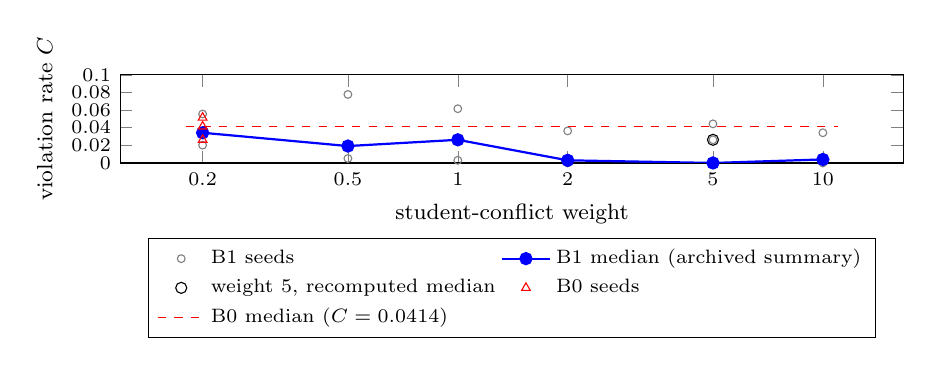
\begin{tikzpicture}
\begin{axis}[
    width=0.95\linewidth, height=2.7cm,
    xmode=log, log basis x=10,
    xtick={0.2,0.5,1,2,5,10},
    xticklabels={0.2,0.5,1,2,5,10},
    xlabel={\footnotesize student-conflict weight},
    ylabel={\footnotesize violation rate $C$},
    ymin=0, ymax=0.10,
    scaled y ticks=false,
    yticklabel style={/pgf/number format/fixed, /pgf/number format/precision=2},
    tick label style={font=\scriptsize},
    legend style={font=\scriptsize, legend columns=2,
        at={(0.5,0)}, anchor=north, yshift=-2.7em},
    legend cell align=left
]
\addplot[only marks, mark=o, color=gray, mark size=1.4pt] coordinates {
 (0.2,0.0343) (0.2,0.0556) (0.2,0.0202)
 (0.5,0.0192) (0.5,0.0051) (0.5,0.0778)
 (1,0.0616) (1,0.0030) (1,0.0263)
 (2,0.0364) (2,0.0030) (2,0.0000)
 (5,0.0263) (5,0.0000) (5,0.0444)
 (10,0.0343) (10,0.0000) (10,0.0040)
};
\addlegendentry{B1 seeds}
\addplot[mark=*, thick, color=blue] coordinates {
 (0.2,0.0343) (0.5,0.0192) (1,0.0263) (2,0.0030) (5,0.0000) (10,0.0040)
};
\addlegendentry{B1 median (archived summary)}
\addplot[only marks, mark=o, mark size=2pt, color=black] coordinates {(5,0.0263)};
\addlegendentry{weight 5, recomputed median}
\addplot[only marks, mark=triangle, color=red, mark size=1.8pt] coordinates {
 (0.2,0.0414) (0.2,0.0263) (0.2,0.0515)
};
\addlegendentry{B0 seeds}
\addplot[dashed, color=red, domain=0.18:11, samples=2] {0.0414};
\addlegendentry{B0 median ($C=0.0414$)}
\end{axis}
\end{tikzpicture}
\caption{Student violation rate against the student-conflict weight on a fixed instance (262 classes, 990 students, 900\,s per run, three seeds per weight). Open circles are the B1 seeds in the per-seed metric files. Triangles are the B0 seeds at weight 0.2 (0.0414, 0.0263 and 0.0515); their median is the dashed line. The black circle at weight 5 is the median recomputed from the files now on disk, 0.0263, rather than the archived summary value of 0. Two B1 seeds remain above 0.06.}
\label{fig:sweep}
\end{figure}

Three things stand out. First, the search does most of the work by itself. From a starting point of $0.5313$, the median of every configuration fell below $0.06$ within the budget, with all 262 classes assigned. Two individual B1 seeds do not: 0.0778 at weight 0.5 and 0.0616 at weight 1. Second, the weight still matters at the margin. Against the B0 median of $0.0414$, weight~2, the best weight on disk, cut the residual rate by $92.7\%$ ($C=0.0030$). The $25\%$ bar in Section~\ref{sec:rl} is a different comparison, a learned policy against a tuned baseline on a held-out instance, and that comparison was not run. In absolute terms there is little left to gain, since $C=0.0030$ is about three conflicted students out of 990. Third, seed noise is large. B0 and B1 at the same nominal weight of 0.2 differ by $17\%$ in their medians ($0.0414$ against $0.0343$). With three seeds per point, differences of that size between neighbouring weights, such as the rise at weight~1, should not be read as real effects.

\subsection{The final solution under pinned enrolments}
\label{sec:final}

By default, UniTime may move a student into a different parallel section to get around a clash. The department assigns laboratory batches administratively, so a lower conflict count achieved this way would describe a cohort structure that does not exist. For the final solve we therefore pinned every student to their section with three settings:

\begin{enumerate}
\item \emph{Student Course Demands} set to \emph{Enrolled Student Course Demands}, so that the solver reads the imported enrolments. Under the default, \emph{Projected Student Course Demands}, a session with no last-like enrolment data loads no students.
\item \texttt{General.SwitchStudents=false}, which turns off the final student-switching pass.
\item \texttt{Global.LoadStudentEnrlsFromSolution=true}, which loads each student's sections from the stored enrolments instead of recomputing them.
\end{enumerate}

With these settings the solver can lower the conflict count only by moving classes. The timetable was solved in session Spr11, exported as \texttt{spr2026\_11\_all\_flags.csv}, and scored in CSV mode against Spr12 (\texttt{0gen\_all}). The two enrolment sets are identical, so the denominator is the same 1{,}130 students.
Table~\ref{tab:final} gives the full evaluation and Fig.~\ref{fig:hardchecks} the hard-check pass rates.

\begin{table}[t]
\centering
\caption{Full evaluation of the final solution (Spr11 export scored in CSV mode against the Spr12 dataset): 291 classes, 1{,}130 students, 42 rooms, 115 staff.}
\label{tab:final}
\footnotesize
\begin{tabular}{@{}lrr@{}}
\toprule
Metric & Value & Rate \\
\midrule
Coverage & 290 / 291 assigned & 99.66\% \\
Hard feasibility score & 98.85 / 100 & --- \\
Hard checks / failures & 4{,}341 / 105 & --- \\
Time-pattern fidelity & 290 / 290 & 100\% \\
Date pattern & 290 / 290 & 100\% \\
Room capacity & 290 / 290 & 100\% \\
Lunch / weekend compliance & 290 / 290 & 100\% \\
Instructor double-booking & 0 conflicts & 100\% \\
Room double-booking & 0 conflicts & 100\% \\
Student conflicts & 40 / 1{,}130 (40 pairs) & 96.46\% \\
Student lunch breaks & 63 violations & 94.42\% \\
Instructor lunch breaks & 1 violation & 97.92\% \\
Travel-time violations & 0 & --- \\
Back-to-back density$^{\S}$ & --- & 31.96\% \\
Unavailable-laboratory usage & 17 / 291 & 5.84\% \\
Preference score$^{\ddagger}$ & 6.29 / 100 & --- \\
\quad room preference & 35 / 278 & 12.59\% \\
\quad instructor identity$^{\dagger}$ & 0 / 289 & 0\% \\
\bottomrule
\end{tabular}
\\[2pt]
\raggedright\footnotesize $^{\ddagger}$Mean of the two rates listed beneath it. $^{\dagger}$Name-format artefact, not a scheduling failure; see Section~\ref{sec:discussion}. $^{\S}$Share of an instructor's consecutive, non-overlapping classes on the same day that meet with no gap.
\end{table}

\begin{figure}[t]
\centering
\resizebox{\linewidth}{!}{%
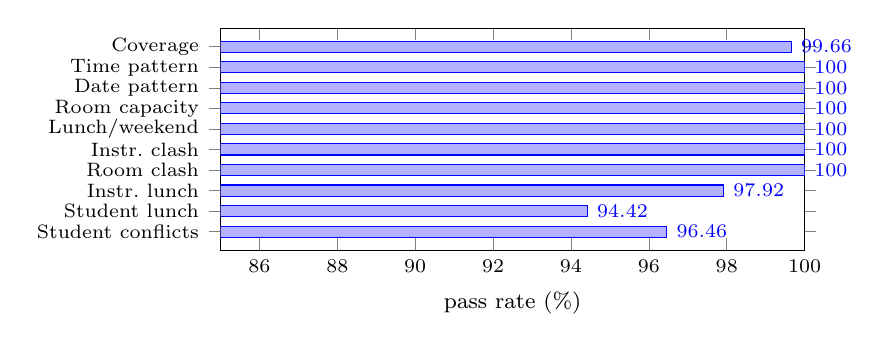
\begin{tikzpicture}
\begin{axis}[
    width=9cm, height=4.4cm,
    xbar, bar width=4pt,
    xmin=85, xmax=100,
    y dir=reverse,
    ytick=data,
    symbolic y coords={Coverage, TimePattern, DatePattern, RoomCapacity, LunchWeekend, InstrClash, RoomClash, InstrLunch, StudentLunch, StudentConflicts},
    yticklabels={Coverage, Time pattern, Date pattern, Room capacity, Lunch/weekend, Instr.\ clash, Room clash, Instr.\ lunch, Student lunch, Student conflicts},
    tick label style={font=\scriptsize},
    nodes near coords, nodes near coords align={horizontal},
    every node near coord/.append style={font=\scriptsize},
    xlabel={\footnotesize pass rate (\%)}, label style={font=\footnotesize}
]
\addplot coordinates {
 (99.66,Coverage) (100,TimePattern) (100,DatePattern) (100,RoomCapacity)
 (100,LunchWeekend) (100,InstrClash) (100,RoomClash) (97.92,InstrLunch)
 (94.42,StudentLunch) (96.46,StudentConflicts)
};
\end{axis}
\end{tikzpicture}}
\caption{Pass rates of the ten hard checks for the final solution. The horizontal axis starts at 85\% so that the four checks below 100\% are legible.}
\label{fig:hardchecks}
\end{figure}

Every requirement the institution treats as non-negotiable holds: 290 of 291 classes are placed, no instructor or room is double-booked, and every placed class keeps its meeting pattern, date pattern and room capacity and stays off weekends. Sixty-three students and one instructor have no free hour in the 11:30--15:30 lunch window; this is a soft criterion, so the solver is allowed to trade it away. Seventeen of the 291 classes (5.84\%) sit in unavailable laboratories taken directly from the official dataset. These laboratories are being
built for these classes and will be usable once operation starts, so the
placements are provisional until then. Placing a class in one of these rooms
does not count as a hard failure

The 40 student clashes are forty first-year students. Eight clash in each of five pairs: CS PPS-FY Lab 1 with FY-Reserve lecture 3, Lab 2 with lecture 3, Lab 7 with lecture 2, and Lab 9 with lectures 1 and 2. The same forty identifiers are in the Spr6 export, but not in these sections. There they sit in PPS-FY labs 1, 2, 5, 6 and 8 (11, 5, 3, 16 and 5 students); lab 9 is not in that file, and none of the forty is in lab 7. A headless zero therefore does not place this sectioning. Re-timing the four laboratories, or a different-time constraint against the reserved lecture, would remove the clashes. Neither remedy has been implemented or measured. Currently 12.59\% of room preferences are satisfied (35 of 278). The historical Taasika room pairings were imported permissively as preferences, so the solver can give them up at little cost. The preference score of 6.29 averages the room-preference rate with the instructor-identity rate, which is 0\% because of a name-format mismatch rather than a scheduling fault (Section~\ref{sec:discussion}).


\subsection{Cross-run comparison}

Table~\ref{tab:crossrun} lists all runs that experienced a conflict and their mode, session and denominator. There are three blocks that should not be read as a continuum: runs made by the UI on the changing Spr6 dataset (CSV mode, 1290 students), the headless sweep on the fixed 990-student dataset (XML mode, end and start), and the pinned-enrolment runs on the 1130 student dataset. Rows should only be compared when the session, mode and student count all match. Therefore comparisons should only be made within a block and not across blocks. Within the UI block (first block) there is no clear trend as the rate varies from 39\% to 69\%. It is also worth noting that weight-20 run is worse than the baseline, a result which Section~\ref{sec:ui-weight} also refuses to interpret. Within the second block (sweep block) the start and end of the sweep seed are reported to be at 2.6\% (26 of 990) and 53.1\% respectively. It is in this section (Section~\ref{sec:weight-sweep}) that the second and final block (pinned block) is introduced. The first pinned run (Spr10, 290 classes, XML mode) gave a conflict rate of 32 of 1130, and the final run (Spr11 against Spr12, 291 classes, CSV mode) gave 40 of 1130. Since the session, classes, and evaluation mode differ, the increase from 32 to 40 should not be interpreted as the timetable getting worse.

The 2.6\% in Block B and the 3.5\% in Block C are not
comparable: they use different instances, denominators and modes.

\begin{table}[t]
\centering
\caption{Evaluated runs with a measured conflict count. CSV mode joins a timetable to an enrolment file; XML mode scores the student block inside a solver file (Section~\ref{sec:evaluator}).}
\label{tab:crossrun}
\scriptsize
\begin{tabular}{@{}llllrrr@{}}
    \toprule
    Run & Mode & Session & Classes & Conflicted & Rate & Hard feas. \\
    \midrule
    \multicolumn{7}{@{}l}{\emph{Block A: UI runs, Spr6-era dataset}} \\
    UI export, v2 & CSV & Spr6 & 260 & 587 / 1{,}290 & 45.5\% & 94.98 \\
    UI export, v3 & CSV & Spr6 & 262 & 507 / 1{,}290 & 39.3\% & 92.66 \\
    UI, weight 5 & CSV & Spr6 & 262 & 676 / 1{,}290 & 52.4\% & 90.97 \\
    UI, weight 20 & CSV & Spr6 & 262 & 894 / 1{,}290 & 69.3\% & 88.96 \\
    \midrule
    \multicolumn{7}{@{}l}{\emph{Block B: headless sweep, fixed instance}} \\
    \multicolumn{7}{@{}l}{\emph{(start and result)}} \\
    Solver export, as loaded & XML & Spr6 & 262 & 526 / 990 & 53.1\% & 92.15 \\
    Sweep B1, $w{=}5$, seed 1 & XML & Spr6 & 262 & 26 / 990 & 2.6\% & 97.42 \\
    \midrule
    \multicolumn{7}{@{}l}{\emph{Block C: pinned enrolments, 1{,}130 students}} \\
    First pinned run & XML & Spr10 & 290 & 32 / 1{,}130 & 2.8\% & 97.77 \\
    Final solution & CSV & Spr11/12 & 291 & 40 / 1{,}130 & 3.5\% & 98.85 \\
    \bottomrule
    \end{tabular}
\end{table}


\section{Reinforcement-Learning Control Experiment}
\label{sec:rl}

The weight sweep of Section~\ref{sec:weight-sweep} tunes one scalar. A bolder question is whether the choice of search move can itself be learned. At each step, CPSolver's neighbourhood selector picks a kind of move (change a time, change a room, swap two classes, ask for a suggestion) according to fixed probabilities. The hypothesis is that a policy conditioned on the state of the search can beat those probabilities and reach a lower student-conflict rate within the same time budget. The success criterion was committed on 28 September 2026 (\texttt{6bf9970}), before the weight sweep of 7 October: a learned policy counts as a success only if it cuts the student violation rate by at least $25\%$ relative to a tuned baseline, at equal wall-clock budget, on a held-out instance.

The search is modelled as a Markov decision process~\cite{sutton2018rl}: an agent observes a state, chooses an action, and receives a reward that depends on where it lands. The agent is consulted once every fifty solver iterations, not at every one, so inference cost stays negligible next to the search itself. The state is a 48-dimensional real vector. It groups conflict features (violation rate, pair rate, intensity, concentration), a ten-bin histogram of conflict load across the day, search-progress features such as acceptance rate and recent improvement slope, solution features (assigned ratio and the normalised room, time and distribution criteria), room and instructor utilisation, and a record of the previous operator chosen. The reward is a potential-based shaping term over the incumbent solution. It folds the student violation rate, the unassigned fraction, the count of hard violations and the normalised soft objective into one scalar, and the step reward is the change in that potential between decision points, minus a small constant that discourages stalling. Potential-based shaping~\cite{ng1999shaping} is chosen because it makes the signal dense without changing the ordering of the final solutions it compares. The trained policy uses proximal policy optimisation~\cite{schulman2017ppo} with invalid actions masked out~\cite{schulte2017maskable}. An online alternative, and not a neural network, is LinUCB~\cite{li2010linucb}, a linear contextual bandit from the upper-confidence-bound family~\cite{auer2002ucb}.

The layer is built on CPSolver's own move-selection extension point, which matters for safety. Nothing in it writes a placement directly. Every candidate move comes from a stock CPSolver generator and then faces CPSolver's own acceptance criterion, exactly as in an ordinary solve. A learned policy can therefore make the search slower or less effective, but it cannot make the timetable illegal. The code base is 25 Java classes and 11 Python modules: a 48-dimensional state encoder; eight neighbourhood operators, six stock CPSolver generators plus two written for this project that bias sampling toward classes and students already in conflict; the potential-based reward term; a gRPC training environment; and an ONNX inference path that runs the frozen policy inside the solver's own Java virtual machine, with a timeout and a fallback to the stock selector. Two of the eight operators, StudentSwap and BiasedStudentSwap, move students between sections, so they must be disabled through \texttt{Rl.DisabledOperators} in any run with pinned enrolments (Section~\ref{sec:final}).

The main comparison was never run, and the project reports this as a null result, not a setback to be explained away. Arm B1 exists to ask whether the stock objective is simply under-weighted, and Section~\ref{sec:weight-sweep} shows that it is. Raising the student-conflict weight on a fixed instance takes the median violation rate from $0.0414$ to $0.0030$ at the best weight (2). That leaves almost no headroom for a learned policy: a $25\%$ gain over $C=0.0030$ means roughly three conflicted students out of 990 becoming two, a difference that three seeds cannot resolve. The only bake-off on a real institutional instance compares the baseline arms alone, and that instance is already conflict-free when loaded, so it could not separate a learned policy from a fixed one even if both ran.

A small synthetic instance (120 classes, 600 students, 6 rooms) does confirm that the training pipeline runs end to end: roughly 100 macro-steps per second per worker, an ONNX forward pass of about 0.08\,ms, and a PyTorch--ONNX numerical deviation of $2\times10^{-6}$. Yet every arm ties at the same violation rate there, and a behaviour-cloned policy is markedly worse, having collapsed onto a single operator. The project's own notes call this a pipeline check, not evidence about search quality, and this paper does the same. The PPO policy was trained on session Spr6 (100{,}000 timesteps, three workers) but was never evaluated on an institutional instance.

Two further points limit how the null result should be read. First, the synthetic check is a pipeline check precisely because the comparison that matters, learned policy against tuned baseline on an institutional instance at a held-out term, is never run. Everything that can be said about search quality on real data rests on Section~\ref{sec:weight-sweep} alone. Second, the layer's design invariant, that every proposed move is still generated and accepted by stock CPSolver machinery, means the worst a mis-trained policy can do is waste search budget. It cannot produce an illegal or materially worse timetable. That is why the layer can stay fully instrumented and only partly evaluated, instead of being withdrawn once the control experiment answers the research question.

No claim is therefore made that the learned policy outperforms the tuned baseline. On this instance, at this budget, the residual conflicts after search come from how the objective is priced, not from how the search explores, and a correctly configured stock solver already suffices. The conflict oracle, state encoder and headless runner built for this layer remain useful regardless. Cross-validating the oracle against the Python evaluator (Section~\ref{sec:evaluator}) is what makes the controlled weight comparison of Section~\ref{sec:weight-sweep} trustworthy in the first place, and the infrastructure is ready should a larger, harder instance resist weight tuning alone.


\section{Discussion}
\label{sec:discussion}

The results above hold under conditions that should be stated plainly rather than left implicit.

\emph{The student body is simulated.} No MIS data was available, so all 1{,}130 students are generated from confirmed headcounts and deterministic enrolment rules rather than actual course choices. Elective demand is modelled as an even split across options, whereas in reality demand is skewed. Under skewed demand, more students would be enrolled in the larger sections, and that would affect which overlaps are of concern. There are also known issues with the way sections were filled to build the simulation. Two postgraduate students overflow one laboratory, and three final-year laboratory batches end up mixed across lecture divisions because the preferred batches of one division filled first. These mixed batches create joint enrolments the institution does not intend, and with them conflict opportunities that a correct section structure would not produce.

\emph{The residual conflicts are diagnosed but not fixed.} The 40 first-year conflicts reported in Section~\ref{sec:final} are localised to four laboratory placements against the reserved lecture block, and two remedies were identified, namely (1) re-timing the laboratories, or (2) adding explicit different-time distribution constraints. However, neither has been implemented or measured, so the number in Table~\ref{tab:final} should be read as a diagnosed and addressable residue rather than a quality ceiling.

\emph{Soft-constraint quality is poor and the preference aggregate is partly uninformative.} The room-preference hit rate of 12.59\% is a genuine optimisation gap: no tuning of the room-preference weight was done, in contrast with the student-conflict weight. The instructor-identity check, on the other hand, has nothing to do with the quality of the schedule and scores 0\%. UniTime exports instructor names in last-name, initial form (``Joshi, A''), while the comparison data uses full names (``Amit Joshi''), so every class fails the identity check. The check needs a name-normalisation step, and until it has one the preference score of 6.29 should not be quoted on its own.

\emph{Scope is one department and one term.} This data represents only Computer Engineering for a single session. A university-wide dataset would span multiple departments and would introduce inter-departmental contention for rooms, which the data here does not exercise.

\emph{The evaluator's own aggregate is a double-edged design choice.} Equal weighting of the checks within each aggregate means that a single structurally broken check can swing the score. For instance, the broken instructor-identity comparison discussed above pulls the preference score down to 6.29 without any change to the underlying schedule. This issue is not unique to this project; any equal-weight aggregation of heterogeneous checks will behave the same way. The only general remedy is the one adopted here, which is to always report the individual check rates alongside the aggregated score.

\emph{Generalisation beyond this instance is untested.} Every number in Sections~\ref{sec:results} and~\ref{sec:rl}, including the weight sweep and the reinforcement-learning control experiment, was measured on one department's data for one term. Nothing in the pipeline is specific to that department, since the generators are parameterised by snapshot and academic term, but no second, independently sized instance was solved and scored end to end during this phase. Claims about how the residual conflict rate or the weight sensitivity would behave on a larger or structurally different instance therefore remain extrapolations rather than measurements.

\emph{Software stack.} For completeness, the UniTime server runs on Java 21. The modules developed in this project, namely the reinforcement-learning module and the headless tools, declare Java 17 as the compile target but run unchanged on Java 21, since bytecode compiled for release 17 is backwards compatible; no component requires a version downgrade.

These notes point in the same direction: the more enduring contribution of this phase is the measurement machinery, namely the independent evaluator, its cross-validated conflict rule, and the pinned-enrolment protocol. Together, they turn the student-conflict count into a small, honest, and diagnosable number that reflects the timetable itself rather than the solver's internal bookkeeping.

\section{Conclusion}
\label{sec:conclusion}
\enlargethispage{6\baselineskip}

A preceding feasibility phase proved that UniTime's constraint model was good enough to capture all the scheduling rules in effect in this department. This phase transformed it into a working system and, in the process, provided a measured schedule rather than a feasibility argument. A reproducible pipeline reads a scheduling database snapshot and generates the 16 ordered documents that UniTime imports for a single session. It covers 42 rooms across six buildings, 115 teachers, 56 offerings, 291 classes and 1{,}130 simulated students with 9{,}148 enrolments. The pipeline includes validators that ensure no archive is generated from inconsistent data. The minor-degree and open-elective time blocks are generated as data rather than entered by hand after each import. The lunch window is not re-entered with them: a Jython script run inside UniTime writes its solver-parameter definitions into the UniTime database before the solver is run. An independent evaluator scores the exported schedules against the same inputs, using a conflict definition cross-validated against an independent implementation to exact numerical agreement.

The main issue is with measurement as much as with optimisation. By default, UniTime can lower the conflict count by moving students between parallel sections, which describes a cohort structure the department does not have. Pinning the enrolments removed that option, so the solver could improve the count only by moving classes, and the conflicts that remain are a property of the timetable itself. The final solution, solved in session Spr11 and scored against the Spr12 dataset, placed 290 of 291 classes with no instructor or room double-booking, giving a hard feasibility score of 98.85 out of 100. Forty of the 1{,}130 students had conflicts, all of them first-year students, arising from four programming-laboratory placements against the reserved first-year lecture block. This is a scheduling problem with a known shape rather than a quality ceiling.

These settings matter because earlier runs without them reported zero student conflicts for reasons unrelated to the timetable. With student switching enabled, the final sectioning pass moved students between parallel laboratory batches until the overlaps disappeared, while the class placements stayed unchanged. Under projected demand, one session loaded no students and reported zero conflicts out of zero. A third run, a baseline bake-off, reported zero in every arm because the instance was already conflict-free when loaded. None of these is a conflict-reduction result, and none is reported as one here.

This project implemented a reinforcement-learning layer that chooses among CPSolver's neighbourhood operators, designed so that it can never output an illegal timetable: every change it proposes is generated and accepted by the stock CPSolver machinery. No claim is made that learning outperforms the tuned baseline. To make this system operational, three changes are needed: 1) a return path from the solved timetable to the live scheduling database, 2) student data obtained from the MIS portal instead of simulation, and 3) an extension of scope to other departments and terms. These changes are well-defined. None of the three is blocked on anything reported here: the pipeline is already parameterised by snapshot and term rather than hard-coded to this department's data, the evaluator already treats the solver as a black box and would score a university-wide export the same way it scores this one, and the remedies for the first-year conflicts have been identified but not yet implemented. The more general lesson, independent of this particular department or dataset, is that a scheduler's self-reported quality metric should never be trusted without an evaluator built to the same standard of independence used here, one that is handed a timetable and a set of enrolments and nothing else, and that therefore cannot be fooled by whatever the solver did internally to arrive at the number it would rather report.

\section*{Acknowledgment}
The authors thank their project guide, Abhijit~A.~M., for supervision throughout this phase, and the department for providing the Taasika database snapshots used throughout this study.

\bibliographystyle{IEEEtran}
\bibliography{references}

\end{document}
